%! Author = joseph
%! Date = 27.04.21
% TODO: save copy as beamer template

\documentclass[a4paper, x11names, svgnames]{beamer}

% -- packages
% encoding, language and fonts, more powerful macros
\usepackage[utf8]{inputenc}
\usepackage[T1]{fontenc}
\usepackage{xargs}
\usepackage{xifthen}
%color
%\usepackage[x11names, svgnames]{xcolor}
% math symbols
\usepackage{amsthm}
\usepackage{amsmath}
\usepackage{amssymb}
\usepackage{amsfonts}
\usepackage{bbding}      % checksymbol
\usepackage{array}       % matrices
\usepackage{multicol}
% roman/ arabic enumeration
% graphics, code
\usepackage{float}
\usepackage{caption}
\usepackage{subcaption}
\usepackage{graphicx}
\usepackage{tikz}
\usetikzlibrary{shapes.misc} % for cross in latex
\usepackage{environ}  % to scale tikz to scale
\usepackage{color}
\usepackage{mathtools}
\usepackage{xcolor}
\usepackage{wasysym}

% package options
\usetikzlibrary{patterns}
\tikzset{cross/.style={cross out, draw=black, minimum size=2*(#1-\pgflinewidth), inner sep=0pt, outer sep=0pt},
%default radius will be 1pt.
    cross/.default={1pt}}  % draw crosses: "\draw (x,y) node[cross=<size>] {};

% -- macros
% Zeichen
\input{~/templates/math_symbols.tex}

% spacing
\newcommand{\offset}{1cm}

% -- enviornments
% english theorem env % TODO: export into single file
\theoremstyle{definition}
\newtheorem*{defn}{Definition}
\theoremstyle{plain}
\newtheorem*{prop}{Proposition}
\theoremstyle{plain}
\newtheorem*{cor}{Corrolary}
%\theoremstyle{remark}
%\newtheorem*{proof}{Proof}

% -- document settings 
\title{Linear Programming}
\subtitle{The Simplex Algorithm}
\author{Joseph Holten}
\date{12.5.2021}

% beamer settings
\usetheme{Hannover}
\usecolortheme{seahorse}
\usefonttheme{professionalfonts}


% beamer pause in align
\makeatletter
\let\save@measuring@true\measuring@true
\def\measuring@true{%
    \save@measuring@true
    \def\beamer@sortzero##1{\beamer@ifnextcharospec{\beamer@sortzeroread{##1}}{}}%
    \def\beamer@sortzeroread##1<##2>{}%
    \def\beamer@finalnospec{}%
}
\makeatother

% ------ DOCUMENT START -------------
\begin{document}

% title frame
\frame{\maketitle}

% TOC
\frame{\frametitle{Overview}\tableofcontents}   % TODO: move toc to right
% TODO: better sections

\section[Preliminaries]{Preliminaries}

% beamer section titles
\AtBeginSection[]{
    \begin{frame}
        \setcounter{tocdepth}{1}
        \frametitle{Section}
        \tableofcontents[currentsection]
    \end{frame}}

% inutition
\subsection[LP Intuition]{Linear Program Intuition}
\begin{frame}{Linear Program Intuition}
    What is a linear Program? $\Ra$ Optimization of a linear function
    \begin{align*}
        \text{1D:} & \qquad &\text{objective} &= c_1\cdot x_1 \\
        \pause
        \text{2D:} & \qquad  & &= c_1\cdot x_1 + c_2\cdot x_2
    \end{align*}
    \pause
    \center
    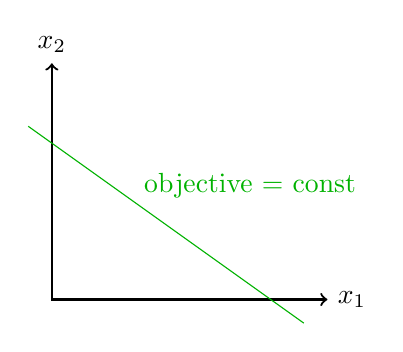
\begin{tikzpicture}
        \draw [<->, thick] (0,3) node (yaxis) [above] {$x_2$} |- (3.5,0) node (xaxis) [right] {$x_1$};
        \draw [black!30!green] (-0.3, 2.2) -- (3.2, -0.3) node [pos=0.35, above, label={right:objective = const}] {};
    \end{tikzpicture}
\end{frame}

% intuition cont.
\begin{frame}{Linear Program Intuition}
        \[c,x \in \R^2\]
        \[\text{objective} = c\cdot x = \textcolor{darkgray}{c^\top x}\]
    \pause
    Constraints:
    \begin{overlayarea}{0.45\textwidth}{0.4\textheight}\visible<3->{ % TODO: align constraints vertically
        \[A \in \R^{2\times 2}, b \in \R^2\]
        \[Ax \leq b\]  % TODO: align =
        \[x \geq 0\]
    }\end{overlayarea}%
    \begin{overlayarea}{0.45\textwidth}{0.4\textheight}  % TODO: single constraints after each other -> system of inequalities = matrix
        \only<2-3>{\center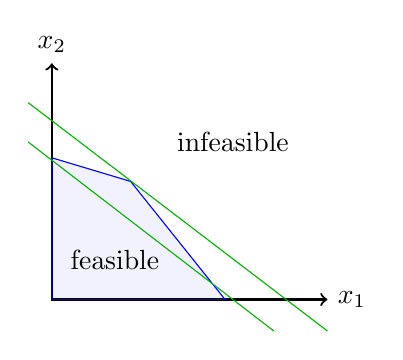
\begin{tikzpicture}
            \draw [<->, thick] (0,3) node (yaxis) [above] {$x_2$} |- (3.5,0) node (xaxis) [right] {$x_1$};
            \draw [blue, fill=blue, fill opacity=0.05] (0.0, 1.8) -- (1, 1.5) -- (2.2, 0.0) -- (0,0) -- cycle;
            \draw [black!30!green] (-0.3, 2.5) -- (3.5, -0.4);
            \draw [black!30!green] (-0.3, 2.0) -- (2.82, -0.4);
            \node at (0.8, 0.5) {feasible};
            \node at (2.3, 2.0) {infeasible};
        \end{tikzpicture}}%
        \only<4>{\center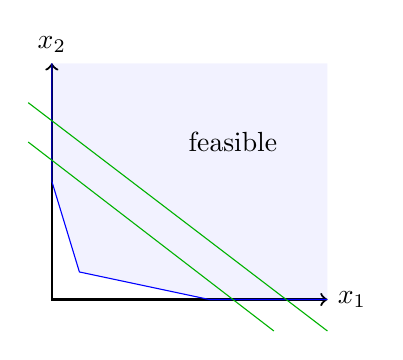
\begin{tikzpicture}
             \draw [<->, thick] (0,3) node (yaxis) [above] {$x_2$} |- (3.5,0) node (xaxis) [right] {$x_1$};
             \draw [blue] (3.5,0) -- (2.0, 0) -- (0.35, 0.35) -- (0, 1.5) -- (0, 3);
             \draw [opacity=0, fill=blue, fill opacity=0.05] (3.5,0) -- (2.0, 0) -- (0.35, 0.35) -- (0, 1.5) -- (0, 3) -- (3.5, 3) -- cycle;
             \draw [black!30!green] (-0.3, 2.5) -- (3.5, -0.4);
             \draw [black!30!green] (-0.3, 2.0) -- (2.82, -0.4);
             \node at (2.3, 2.0) {feasible};
        \end{tikzpicture}}
    \end{overlayarea}
\end{frame}

% 3D example
\begin{frame}{Linear Program Intuition}
    In 3D:
    \begin{figure}
        \center
        \includegraphics[scale=0.5]{3dpoly.svg}
    \end{figure}
    \center\vfill\tiny\textit{\textcolor{gray}{$\langle$en.wikipedia.org/wiki/Linear\_programming$\rangle$}}
\end{frame}

% definition
\subsection[LP Definition]{Linear Program Definition}
\begin{frame}{Linear Program Definition}
    \begin{defn}[Linear Program]
        A \textbf{Linear Program (LP)} is the following optimization problem: \\
        \vspace*{0.3cm}
        \hspace*{0.5cm}Given $A \in \R^{n\times m}, b \in \R^m, c\in\R^n$  \\
        %\vspace*{0.7cm}
        \hspace*{1.5cm}  % TODO: position table
        \begin{tabular}{l l}
            find        & $x \in\R^n$  \\  % TODO: possible center aligned text in 2nd column
            maximizing  & $c\cdot x$   \\
            s.t.        & $Ax \leq b$  \\
        \end{tabular} \\
        \pause
        \vspace{0.3cm}
        Special cases: \\
        \begin{itemize}
            \item $\{x\st Ax\leq b\}$ empty
            \item unbounded: $\forall\alpha\in\R\,\exists x\in\R^n\st c\cdot x > \alpha$
        \end{itemize}
        The set $\{x \st Ax \leq b\}$ is called a \textbf{polyhedron}.
        A bounded polyhedron called a polytope.
    \end{defn}
\end{frame}

%% feasible + bounded => has opt
%\begin{frame}{Existance of Optimum}
%    \begin{theorem}
%        If a Linear Program is feasible and bounded, there is a vector attaining the maximum. \\
%        \pause
%        Formally: For $P=\{x\in\R^n\st Ax\leq b\}\neq\emptyset$ and $c\in\R^n$
%        with $\delta\coloneqq\sup\{c\cdot x\st x\in P\} < \infty$. Then there exists a vector $z\in P$
%        with $\delta = c\cdot z$.
%    \end{theorem}
%\end{frame}

% properties of polyhedra
\subsection{Polyhedra}
\begin{frame}{Polyhedrea}
    % definitions
    \begin{minipage}[l]{0.6\textwidth}
    \begin{defn}
        Let $P\coloneqq\{x\st Ax \leq b\}$ be a (non empty) polyhedron.
        \vspace{0.2cm}
        \begin{itemize}
            \item<2-> For $c\in\R^n \setminus \{0\}$ with $\delta \coloneqq\max\{c\cdot x\st x\in P\}$ finite,
                      then $\{x\st c\cdot x = \delta\}$ is a supporting \textbf{hyperplane}.
            \item<3-> $P \cap \text{hyperplane}$ is a \textbf{face}.
            \item<4-> If $\{x\}$ is a face, x is called a \textbf{vertex}.
        \end{itemize}
    \end{defn}
    \end{minipage}
    % picture
    \begin{minipage}[r]{0.35\textwidth}
        \resizebox{\textwidth}{!}{
        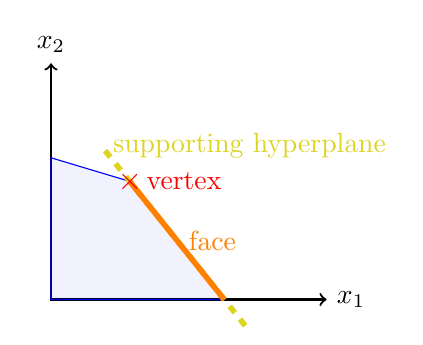
\begin{tikzpicture} % TODO: overlapping lines not pretty
            % axis
            \draw [<->, thick] (0,3) node (yaxis) [above] {$x_2$} |- (3.5,0) node (xaxis) [right] {$x_1$};
            % polygon
            \draw [blue, fill=blue, fill opacity=0.05] (0.0, 1.8) -- (1, 1.5) -- (2.2, 0.0) -- (0,0) -- cycle;
            % polygon missing one side
            %\draw<2-> [blue] (0.0, 1.8) -- (1.5, 1.2);
            %\draw<2-> [blue] (2.5, 0.0) -- (0,0);
            %% fill
            %\draw<2-> [opacity=0, fill=blue, fill opacity=0.05] (0.0, 1.8) -- (1.5, 1.2) -- (2.5, 0.0) -- (0.0, 0.0) -- cycle;
            %% single side low opacity
            %\draw<2>  [blue, opacity=0.2] (1.5, 1.2) -- (2.5, 0.0);
            % supporting hyperplane
            \draw<2->  [black!15!yellow, dashed, shorten >=-0.5cm, shorten <=-0.5cm, line width=2pt] (1, 1.5) -- node[pos=-0.3, right] {supporting hyperplane} (2.2, 0.0) ;
            % face
            \draw<3-> [orange, line width=2pt] (1.0, 1.5) -- node[pos=0.5, right] {face} (2.2, 0.0);
            % vertex
            \node<4-> [cross=3pt, label=right:\textcolor{red}{vertex}, red] at (1, 1.5) {};
        \end{tikzpicture}}
    \end{minipage}
\end{frame}

% prop face = solution of subsystem
\begin{frame}{Characterisation of Faces}
    \begin{prop}
        Let $P=\{x\st Ax\leq b\}$ and $F \subset P$. \\
        Then $F$ is a face of $P \iff F=\{x\in P\st A'x=b'\}\neq\emptyset$ for some subsystem $A'x\leq b'$ of $Ax\leq b$.
    \end{prop}
    \center
    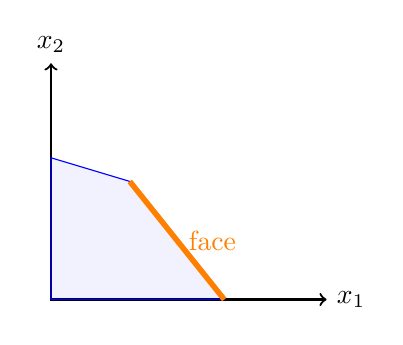
\begin{tikzpicture}
        % axis
        \draw [<->, thick] (0,3) node (yaxis) [above] {$x_2$} |- (3.5,0) node (xaxis) [right] {$x_1$};
        % polygon
        \draw [blue, fill=blue, fill opacity=0.05] (0.0, 1.8) -- (1, 1.5) -- (2.2, 0.0) -- (0,0) -- cycle;
        \draw [orange, line width=2pt] (1.0, 1.5) -- node[pos=0.5, right] {face} (2.2, 0.0); % TODO: no double lines
        % vertex
    \end{tikzpicture}
\end{frame}

% face is maximum
\begin{frame}{Characterisation of Faces}
    \begin{cor}
        For a polyhedron $P\coloneqq \{x\st Ax\leq b\}$ and a LP $\max\{c\cdot x\st x\in P\}$,
        the set of points attaining the maximum, are a face of $P$.
    \end{cor}
    \begin{minipage}[l]{0.55\textwidth}
        \center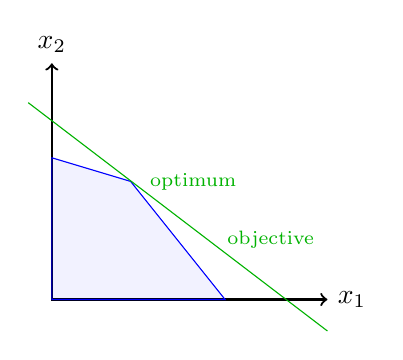
\begin{tikzpicture}
            \draw [<->, thick] (0,3) node (yaxis) [above] {$x_2$} |- (3.5,0) node (xaxis) [right] {$x_1$};
            \draw [blue, fill=blue, fill opacity=0.05] (0.0, 1.8) -- (1, 1.5) -- (2.2, 0.0) -- (0,0) -- cycle;
            \draw [black!30!green] (-0.3, 2.5) -- node[pos=0.6, label=right:{\scriptsize objective}] {} (3.5, -0.4);
            \node [label=right:{\scriptsize \textcolor{black!30!green}{optimum}}] at (1, 1.5) {};
        \end{tikzpicture}
        \center \small Vertex
    \end{minipage}\begin{minipage}[r]{0.35\textwidth}
        \center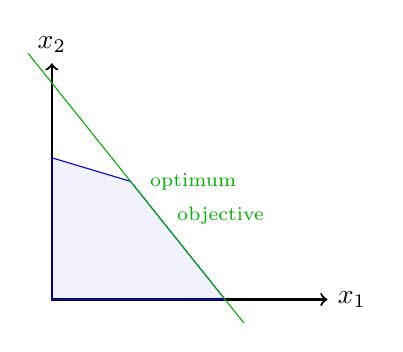
\begin{tikzpicture}
            \draw [<->, thick] (0,3) node (yaxis) [above] {$x_2$} |- (3.5,0) node (xaxis) [right] {$x_1$};
            \draw [blue, fill=blue, fill opacity=0.05] (0.0, 1.8) -- (1, 1.5) -- (2.2, 0.0) -- (0,0) -- cycle;
            \draw [black!30!green] (-0.3, 3.125) -- node[pos=0.6, label=right:{\scriptsize objective}] {} (2.44, -0.3);
            \node [label=right:{\scriptsize \textcolor{black!30!green}{optimum}}] at (1, 1.5) {};
        \end{tikzpicture}
        \center \small Face
    \end{minipage}
\end{frame}


\section{Duality}
% duality
\subsection{Definition}
\begin{frame}{Definition}
    \center{Inside $\Ra$ Outside}
    \begin{figure}
        \center
        \includegraphics[scale=0.28]{duality}
        \vfill\center\scriptsize\textcolor{gray}{$\langle$http://www.science4all.org/article/simplex-methods$\rangle$}
    \end{figure}
\end{frame}

\begin{frame}{Duality Definition}
    \begin{defn}
        Given a LP $\max\{c\cdot x\st Ax\leq b\}$ (called the \textbf{primal LP}),
        the \textbf{dual LP} is the linear program $\min\{y\cdot b\st y^\top A =c, y\geq 0\}$.
    \end{defn}

\end{frame}

% duality prop & theorem
\subsection[Central Theorem]{Central Theorem of Duality}
\begin{frame}{Duality}
    \begin{prop}
        The dual of the dual of an LP is (equivalent to) the primal LP.
    \end{prop}
    \pause
    \begin{theorem}[Duality Theorem]
        If the primal and it's dual LP are feasible, their solutions are the same. \\
        Formally: If $P\coloneqq\{x\st Ax\leq b\}$ and $D\coloneqq\{y\st y^\top A=c, y\geq 0\}$ are non empty,
        then \[\max\{c\cdot x\st x\in P\}=\min\{y\cdot b\st y\in D\}.\]
    \end{theorem}
\end{frame}

\subsection{Weak Duality}
\begin{frame}{Duality}
    \begin{prop}[Weak Duality]
        Let $x$ and $y$ be feasible solutions of the LP's $\max\{c\cdot x \st Ax \leq b\}$
        and $\min\{y\cdot b\st y^\top A = c, y\geq 0\}$.
        Then $c\cdot x \leq y \cdot b$.
    \end{prop}
\end{frame}


\section[Simplex]{The Simplex Algorithm}
\subsection{Intutition}
\begin{frame}{Simplex Algorithm Intuition}
    Let $c=\begin{pmatrix*}0,0,1\end{pmatrix*}^\top$, and $P=\{x\st Ax\leq b\}$ a dodecahedron
    Simplex Algorithm on $\max\set{c\cdot x \st Ax \leq b}$:

    \begin{figure}
        \center
        \includegraphics[scale=0.15]{simplex_walking}
    \end{figure}
    \center\vfill\tiny\textit{\textcolor{gray}{Oliver Friedmann, researchgate.net/figure/Simplex-algorithm-walking-along-the-edges-of-an-LP-polytope\_fig2\_267255049}}
\end{frame}

\subsection{Algorithm}
\begin{frame}{Simplex Algorithm}
    \begin{description}
        \item[\textit{Input:}] a linear program $\max\set{x\st x\in P}$, for  $P\coloneqq \set{x\st Ax \leq b}$ and a vertex $x$ of the polyhedron $P$ . \\
        \item[\textit{Output:}] vertex $x$ attaining the $\max\set{c\cdot x \st x\in P}$, or a vector $w$ in a direction in which the LP is unbounded.  \\
    \end{description}
    \vspace{0.6cm}
    Define for $J$ a set of row indices the submatrix $A_J$, analogously $b_J$ and $a_i \coloneqq A_{\set{i}}$ (the $i$'th row of $A$), $b_{i}\coloneqq b_{\set{i}}$.
\end{frame}

\begin{frame}{Simplex Algorithm}
    \textit{Algorithm:}
    \begin{enumerate}
        \item \label{step:1}Choose a set of n row indices $J$ such that $A_J$ is invertible and $A_{J}x = b_J$.
        \pause
        \item \label{step:2} Compute $c^\top (A_J)^{-1}$ and add zeros to obtain a vector $y$ with $c^\top = y^\top A$,
        such that all entries of $y$ outside $J$ are zero. \\
        \textbf{If} $y\geq 0$ \textbf{then stop. Return} $x$ and $y$.
        \pause
        \item  \label{step:3}Choose the minimum index $i$ with $y_i < 0$. \\
        Let $w$ be the column of $-(A_J)^{-1}$ with index $i$, so $A_{J\setminus\{i\}}w=0$
        and $a_i \cdot w = -1$.
        \pause
        \item \label{step:4}Let $\lambda \coloneqq \min  \set{\frac{b_j - a_j\cdot x}{a_j\cdot w} \st j\in\set{1,\dots, m}, a_j\cdot w > 0}$,
        and let $j$ be the smallest row index attaining this minimum.
        \pause
        \item \label{step:5} Set $J\coloneqq (J\setminus\set{i})\cup \set{j}$ and $x\coloneqq x + \lambda w$. \\
        \textbf{Go to}~\ref{step:2}.
    \end{enumerate}
\end{frame}

\begin{frame}{Simplex Algortihm Theorem}
    \begin{theorem}
        \begin{itemize}
            \item<1-> Termination in at most $\binom{m}{n}$ iterations.
            \item<2-> $x$ and $y$ returned in step~\ref{step:2} are optimum solutions of the LP and its dual.
            \item<3-> $w$ returned in step~\ref{step:3} is a direction in which the LP is unbounded.
        \end{itemize}
    \end{theorem}
\end{frame}
\subsection{Proof}

\begin{frame}{Simplex Algorithm correctness}
    \begin{proof}
        First we will show the algorithm terminates.
        To follow closely, please refer to the algorithm on p. 57 of Combinatorial Optimization by Korte and Vygen. \\ %TODO: correct citation, make grey and italic?
        Invariants:
        \renewcommand{\theenumi}{(\alph{enumi})}
        \begin{multicols}{3}
        \begin{enumerate}  % TODO: labels
            \item $x \in P$
            \item $A_J x = b_J$
            \item $A_J$ invertible
            \item $c\cdot w > 0$
            \item $\lambda \geq 0$
        \end{enumerate}
        \end{multicols}

    \end{proof}  % TODO: beamer proof no qed symbol (custom proof env without?)
\end{frame}


\linespread{1.5}
\begin{frame}{Simplex Algorithm termination}
    \begin{proof}
        Since $|J| = n$ and $J\subset\set{1,\dots, m}$ \\ $\Ra$ number of possible cominations $=\binom{m}{n}$. \\
        Doesn't terminate in $\binom{m}{n} \Ra \exists \text{ iterations } k, l\st J^{(k)}=J^{(l)}$. \\
        By (b), (c) $\Ra x^{(k)}=x^{(l)}$. \\
        Since $x^{(i+1)}\coloneqq x^{(k)}+\lambda w$ and (d): $c\cdot w > 0$ and (e): $\lambda \geq 0$, $c\cdot x$ non decreasing (strictly increasing for $\lambda > 0$). \\
        Thus $\lambda = 0$ for $k, \dots, l-1$ and $x^{(k)} = \dots = x^{(l-1)}$. \\
    \end{proof}
\end{frame}

\begin{frame}{Simplex Algorithm termination}
    \begin{proof}
        Let $h$ be the highest index removed from $J$ in iterations $k, \dots, l-1$ say in iteration $p$.
        $h$ was added in a iteration $q \in \set{k, \dots, l-1}$ since $J^{(k)}=J^{(l)}$ (what leaves must have been added). \\
        Define $y'\coloneqq y^{(p)}, w'\coloneqq w^{(q)}$.
        Know $c=y'^\top A$ $\Ra y'^\top A w' = c^\top w' > 0$ ($*$). \\
    \end{proof}
\end{frame}

\begin{frame}{Simplex Algorithm termination}
    \begin{proof}
        Let $r$ be index s.t. $y'_r a_r w' > 0$
        Since $y'_r \neq 0 \Ra r\in J^{(p)}$. If $r > h \Ra r\in J^{(k)}, \dots, J^{(l-1)}$ (otherwise violating construction of $h$).
        Thus $a_r \cdot w' = 0$ contradicting the choice of $r$, so $r \leq h$.
        It is evident, that $a_r \cdot w' >0 \iff r=h \iff y'_r < 0$, contradicting ($*$).
    \end{proof}
\end{frame}


\begin{frame}{Simplex Algorithm correctness}
    \begin{proof}
    \renewcommand{\theenumi}{(\alph{enumi})}
    \begin{enumerate}
        \item After step~\ref{step:4} it holds that $A_{J\setminus\set{i}}w=0$ and $\lambda = \frac{b_j-a_j\cdot x}{a_j\cdot w}$
            $\Ra A_{J\setminus\set{i}}(x+\lambda w) = A_{J\setminus\set{i}}x + 0 = b_{J\setminus\set{i}}$
            and $\Ra a_j\cdot (x+\lambda w) = a_j \cdot w + \frac{b_j - a_j\cdot x}{a_j\cdot w} a_j\cdot w = b_j$. \\
            Thus $A_{(J\setminus\set{i})\cup\set{j}}(x+\lambda w) = b_{(J\setminus\set{i})\cup\set{j}}$.
    \end{enumerate}
    \end{proof}
\end{frame}

\begin{frame}{Simplex Algorithm correctness}
    \begin{proof}
        \renewcommand{\theenumi}{(\alph{enumi})}
        \begin{enumerate}[(b)]
        \item show $x \in P \Ra x + \lambda w \in P$. Let $k$ be a row index.\\
            Two cases: % TODO: proper cases
            $a_k\cdot w \leq 0$\\
            $\Ra a_k\cdot (x+\lambda w) = a_k\cdot x + a_k\cdot w \leq a_k\cdot x \leq b_k$ \\
            $a_k \cdot w \geq 0$ \\
            Since $\lambda \coloneqq \min  \set{\frac{b_i - a_j\cdot x}{a_j\cdot w} \st j\in\set{1,\dots, m}, a_j\cdot w > 0}$ \\
            then $k$ in considered indices $\Ra \lambda \leq \frac{b_k - a_k\cdot x}{a_k\cdot w} $
            $\Ra a_k\cdot (x + \lambda w) \leq a_k\cdot x + \frac{b_k-a_k\cdot x}{a_k\cdot w} a_k\cdot w  = b_k$. \\
            Therefore in both cases $\Ra x+\lambda w \in P$.
        \end{enumerate}
    \end{proof}
\end{frame}

\begin{frame}{Simplex Algorithm correctness}
    \begin{proof}
        \renewcommand{\theenumi}{(\alph{enumi})}
        \begin{enumerate}[(c)]
        \item $A_J$ invertible, is $A_{(J\setminus\set{i})\cup\set{j}}$? \\
            By step~\ref{step:3} $A_{J\setminus\set{i}} w = 0$ and $a_i w = -1$ for $w$ as $i$'th column of $-(A_J)^{-1}$.
            Iterate over $i$, get $-I_n$ (identity matrix). \\
            After step~\ref{step:4} and~\ref{step:5} $i \leadsto j$ and $a_j w > 0$ $\Ra A_J$ invertible. \\
        \end{enumerate}
    \end{proof}
\end{frame}

\begin{frame}{Simplex Algorithm correctness}
    \begin{proof}
        \renewcommand{\theenumi}{(\alph{enumi})}
        \begin{enumerate}[(d)]
        \item By step~\ref{step:2}: $c^\top=y^\top A$
            $\Ra c\cdot w = c^\top w = (y^\top A)w = y^\top (Aw)$ \\
            and by step~\ref{step:3} $A w = \colvec{0,\dots,-1,0,\dots,0}^\top$
            $\Ra y^\top (Aw) = -y_i > 0$ \pause  \\
    \end{enumerate}
    \end{proof}
\end{frame}

\begin{frame}{Simplex Algorithm correctness}
    \begin{proof}
        \renewcommand{\theenumi}{(\alph{enumi})}
        \begin{enumerate}[(e)]
            \item By step~\ref{step:4} $a_j\cdot w > 0$ and if $x\in P$ then $b_i \geq a_i\cdot x$
            $\Ra \lambda = \frac{b_j-a_j\cdot x}{a_j\cdot w} \geq 0$ for chosen $j$. \\
        \end{enumerate}
    \end{proof}
\end{frame}


\begin{frame}{Simplex Algorithm correctness}
    \begin{proof}
        Invariants hold. \\
        Returning in step~\ref{step:2}: $x$ and $y$ are feasible and from weak duality it follows $x$ and $y$ are optimum. \\
        Returning in step~\ref{step:3}: know $Aw \leq 0$ and $x \in P$. Thus $\forall\mu > 0\st A(x+\mu w) = Ax + \mu Aw \leq Ax \leq b$ $\Ra x+\mu w \in P$
        With (d): $c\cdot w > 0$ it follows that $c\cdot (x+\mu w)$ arbitrarily large, i.e. the LP is unbounded.
    \end{proof}
\end{frame}

\linespread{1.1}

\section[Ellipsoid]{The Ellipsiod Method}

\begin{frame}{Ellipsoid Method Idea}
    \begin{theorem}[Kachiyani]
        From a polynomial-time procedure deciding whether an LP is feasible,
        we can give a polynomial-time algorithm finding the optimum solution.
    \end{theorem}
    \pause
    \vspace{0.5cm}
    Idea of the Ellipsoid method:
    \begin{enumerate}
        \item Take a large ball, containing all feasible solutions.
        \item \label{ellipstep:2} If the center is feasible. \textbf{Return} center.
        \item Otherwise, divide ellipsoid in half through the center, with all feasible solutions on one side.
        \item Calculate smallest ellipsoid containing the feasible half. \textbf{Goto step}~\ref{ellipstep:2}.
    \end{enumerate}
\end{frame}

\begin{frame}{Ellipsoid Visualization}
    \begin{figure}
        \center
        \includegraphics[scale=0.3]{ellipsoid_method_no_text} % TODO: maybe indicate where the feasible region actually is, maybe whiten out the labels
        \vfill
        \tiny\textcolor{gray}{Combinatorial Optimization: Berhnhard Korte, Jens Vygen (p. 83)}
    \end{figure}
\end{frame}

\begin{frame}{Ellipsoid Defintion}
    \begin{defn}
        An \textbf{ellipsoid} is a set
        \[E(A,x) = \set{z\in\R^n\st (z-x)^\top A^{-1}(z-x) \leq 1}\]
        for a symmertric positive definite $n \times n$ matrix $A$. \\
        \pause
        \vspace{0.3cm}  % in a different color?
        Recap: A symmetric positive definite Matrix $A$, is a matrix, fulfilling the following:
        \begin{itemize}
            \item $A = A^\top$ (symmetry)
            \item all eigenvalues are strictly positive $\iff x^\top A x > 0 \quad \forall x\in\R^n \setminus\set{0}$ (positive defniteness)
        \end{itemize}
    \end{defn}
    \pause
    \begin{example}
        $E(r^2 I, x)$ (for $I$ the identity matrix) is an $n$-dimensional Ball with radius $r$.
    \end{example}
\end{frame}

\begin{frame}{Ellipsoid Method formally}
    \begin{prop}[Löwner-John Ellipsoid]
        Given Ellipsoid $E(A,x)$ and a hyperplane $H\coloneqq \set{z\st a\cdot z = a\cdot x}$ (going through x),
        the smallest ellipsoid $E(A', x')$ containing the half-ellipsoid $E\cap H$ is given by:
        \begin{align*}
            A' &= \frac{n^2}{n^2-1} \left( A - \frac{2}{n+1}bb^\top \right) \\
            x' &= x + \frac{1}{n+1}b \\
            b  &= \frac{1}{\sqrt{a^\top A a}} Aa \\
        \end{align*}
    \end{prop}
    Taking care calcualting b to neccessary precision.
\end{frame}

\begin{frame}{Ellipsoid Visualization}
    \begin{figure}
        \center
        \includegraphics[scale=0.3]{ellipsoid_method} % TODO: maybe indicate where the feasible region actually is, maybe whiten out the labels
        \vfill
        \tiny\textcolor{gray}{Combinatorial Optimization: Berhnhard Korte, Jens Vygen (p. 83)}
    \end{figure}
\end{frame}

\begin{frame}
    \Huge Thank you for your attention
\end{frame}

\end{document}
